\documentclass[12pt,a4paper,titlepage]{report}

\usepackage[utf8x]{inputenc}
\usepackage{ucs}
\usepackage[english]{babel}
\usepackage{caption}
\usepackage{xspace}% For a variable space after a macro.
\usepackage{amsmath}
\usepackage[round]{natbib}
\usepackage{amsfonts}
\usepackage{amssymb}
\usepackage{wrapfig}
\usepackage[textsize=large]{todonotes}
\usepackage{graphicx}
\usepackage[left=2cm,right=2cm,top=2cm,bottom=2cm]{geometry}

\bibliographystyle{plainnat}

\author{A.J. Bonnema}
\title{Architecture document}

\begin{document}

\maketitle

\newcommand{\w}[1]{\textsc{#1}}%
\newcommand{\Noc}{\textsc{NoC}\xspace}% 
\newcommand{\xmas}{\textsc{XMas}\xspace}%
\newcommand{\fltk}{\textsc{fltk}\xspace}%
\newcommand{\boost}{\textsc{Boost}\xspace}%
\newcommand{\opengl}{\textsc{OpenGL}\xspace}%
\newcommand{\qt}{\textsc{Qt}\xspace}%
%\newcommand{\code}[1]{\verb%#1%}%
\newcommand{\code}[1]{\texttt{#1}}%
\newcommand{\qobj}{\code{Q\_OBJECT}}%

\chapter{Introduction}

\paragraph{Document use} The document is meant for
developers new to this project and for maintainers
considering a change. It allows a high level view 
and drilling down some to isolate the 
partition that needs change. Finally, the document
is for programmers looking for design guidelines.

\paragraph{Document structure} The document consists
of the high level class diagrams, some sequence diagrams,
some design patterns and finally the design guidelines and 
specific platform dependencies.

\paragraph{Document maintenance} Some of the diagrams -- especially 
the introductory architectural drawings -- were created with \w{Dia}\footnote{you 
can find \w{Dia} at http://sourceforge.net/projects/dia-installer/}.

Most of the \w{UML} diagrams we created with \w{Umbrello}. Be careful to use the most 
recent version as possible. From the the menu option \w{export all diagrams as
picture} or the equivalent option for one diagram one can create an image for
this document.

\paragraph{Naming} Make sure to create names without spaces so the exported filenames
will also be valid. Even though most OS's can work around spaces they
still are a pain to work with. 



\chapter{Architecture Overview}

\section{Partitioning}

\begin{center}
	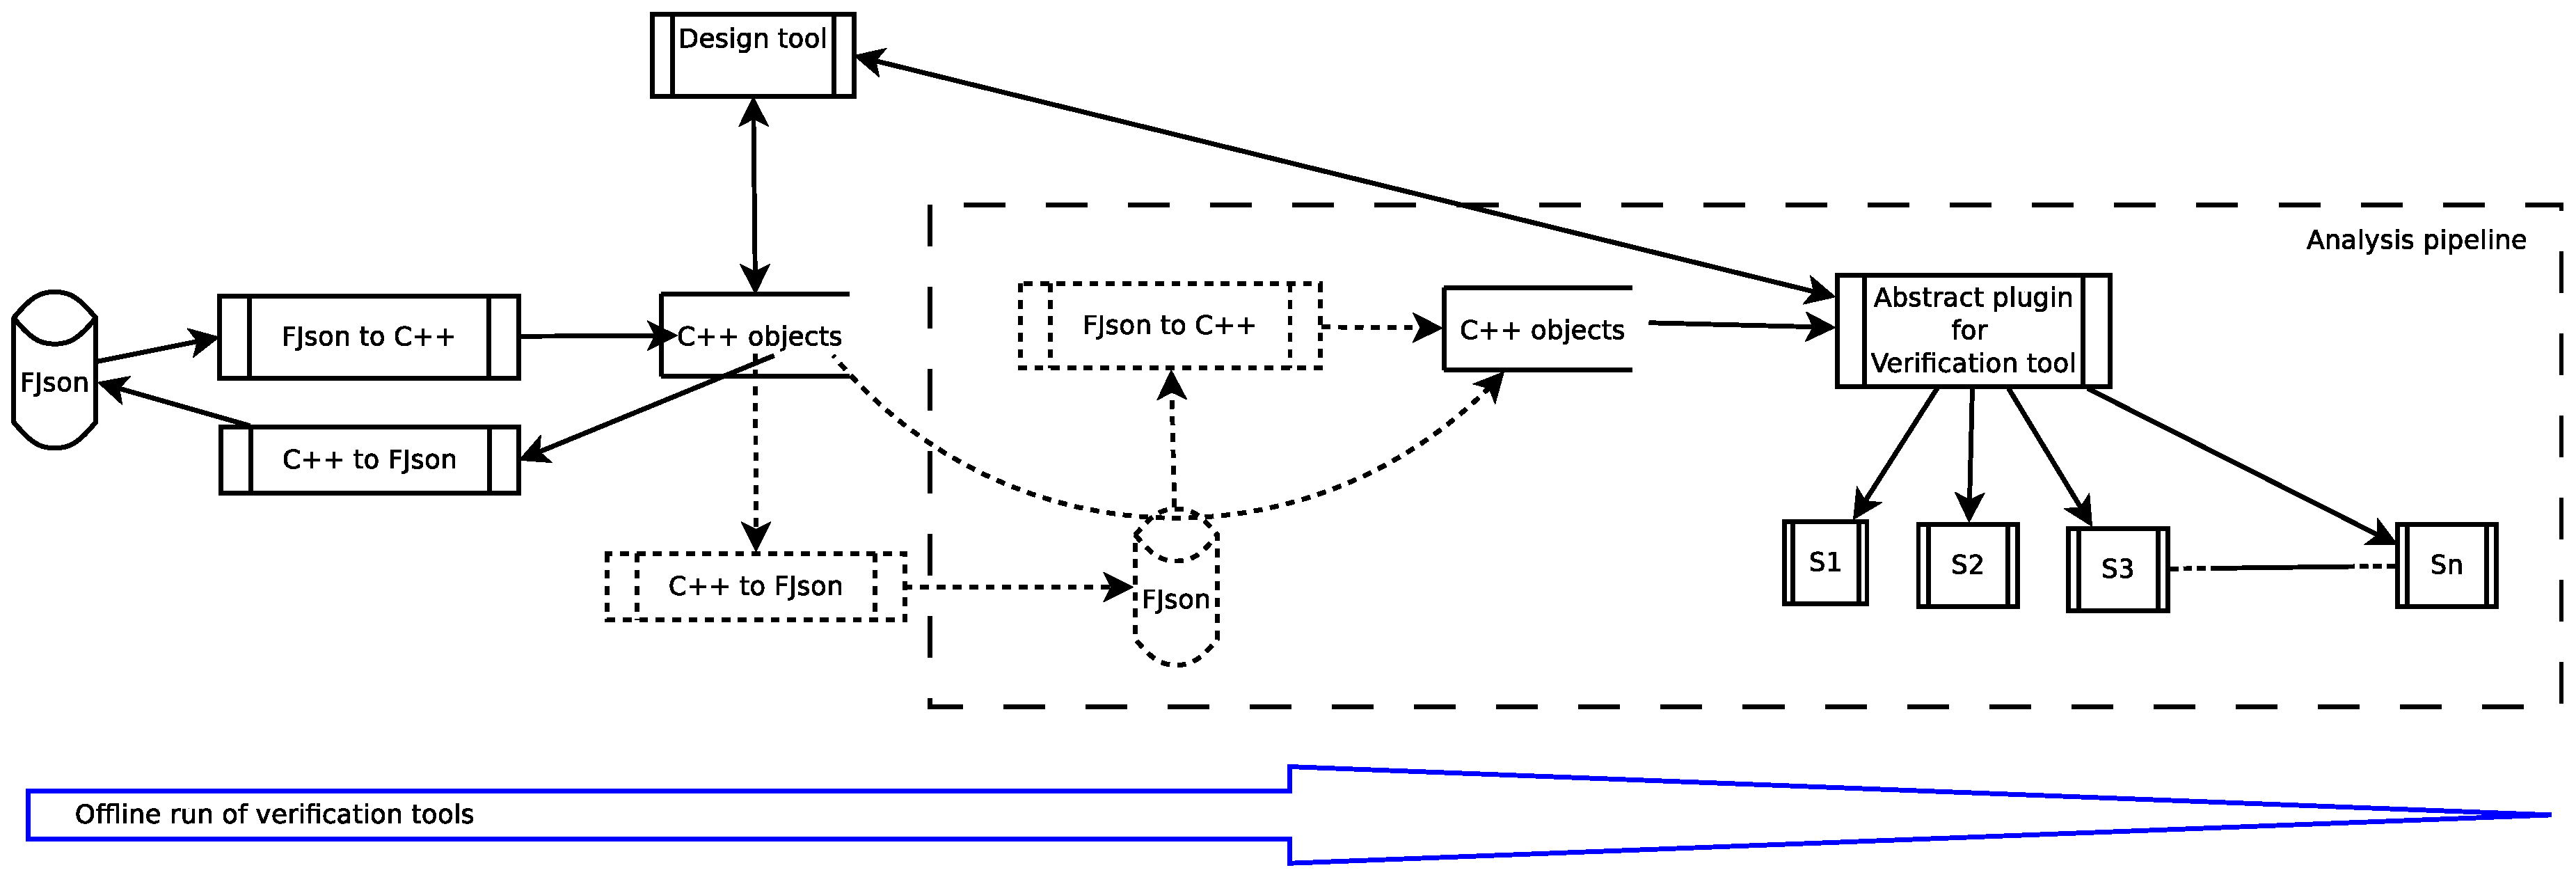
\includegraphics[width=.9\linewidth]{architecture-tool-scope}
\end{center}

The complete tool consists of a verification pipeline and
the graphical user interface where the research people
can design a Network on Chip (\Noc). Both partitions have differing
use cases. 

The use case for the verification pipeline is for verifying a model 
that needs a final check, or for verifying a model that is too 
big to verify completely during graphical edit cycles.

The use case for the graphical editor is for creating, modifying 
and intermediately verifying the \Noc. The editor allows for 
selecting verification tools to run, and will verify parameters
before each run.

The verification tools and the graphical toolkit communicatie 
through a plugin architecture.

\section{Graphical Design Tool}

The graphical editor of \Noc consists of a toolkit containing
the \xmas primitives, the composites available in separate 
libraries, and the graphical window, and the commands to 
prepare and execute the verification tools.

The process of designing an \Noc consists of alternating edit-verify cycles.
Once the model is finished, all parameters per component are filled in, the 
verify tools are selected, the the controller will copy the current model and
kick off the verification tools for an execution run.

\begin{center}
	\includegraphics[width=.9\linewidth]{../architecture-dynamic}
	\captionof{figure}{Dynamic process of editing and verifying}
	\label{fig:dynamic-arch}
\end{center}

\section{Verification pipeline}

For the graphical editor the verification pipeline itself is
not in scope. The connection to the verification pipeline is through
the plugin architecture, where a plugin is wrapped in a C++ class
that derives from \w{VerificationTool}.

Each verification tool must register with the \w{VTController} or 
the controller. The registration involves informing the
\w{VTController} about function, and parameters of the 
verification tool at hand. The graphical editor will ask the 
\w{VTController} for available verification tools.


\section{Layer architecture}

\section{Plugin communication}

\section{Primitive toolkit communication}

\section{Toolkit repository}

\section{Model repository}

\chapter{Architecture Design Guidelines}

\section{Leading requirements}

The following list of leading requirements is meant to guide the creation and maintenance
of design guidelines and design decisions. The most important requirements are first
and foremost leading arguments in any comparison of alternatives. 

\begin{description}

	\item[Portability leads] We need the design tool to run equally well on all defined platforms
	and possibly platforms not (yet) defined. For that reason portability is a leading requirement.
	
	\item[Ease of use seconds] We need the design tool to assist in the design of \Noc and
	the development of verification tools with respect to \Noc designs. For that reason the design
	tool should facilitate these activities as much as possible. 
	
	\item[Maintainability third] The ease of maintenance was one of the primary requirements and
	as such should guide future design decisions. 
	
	\item[Performance follows] Under normal circumstances performance arguments should not lead.
	However, unacceptable performance will override all other considerations, because
	unacceptable performance disrupts use of the tool. 
	
	\item[Remark] What is acceptable performance is subjective. 
	
\end{description}

\paragraph{Example} When given a choice between alternatives with equal portability and 
ease of use consequences, the maintenance arguments should lead at the cost of performance 
provided the performance seems acceptable.

\paragraph{Agreement} On 6th December 2014 Bernard agreed to this priority ordering. 

\section{High level design guidelines}

\begin{description}

	\item[C++ constructs lead] We strive to use C++ of the latest standard, currently C++ 2011.
	This implies the use of the C++ library including containers.
	
	\item[qt] We use the GUI library \qt for all GUI code and as much other code as is necessary.
	
	\item[OpenGL] For drawing 2D we use qtquick1 with graphicsview or qtquick2 which works with opengl.
	It looks like we will be using qtquick1 with graphicsview due to some missing features (scrol, zoom, 
	pan) in qtquick2.

	\item[Other libraries] We use \qt as our goto library for portability. For mechanisms that would
	otherwise require platform dependent code we use \qt. Messaging, process control and
	interprocess communication is all directed through \qt. Only if \qt does not suffice do we
	use other libraries like \boost.
	
	
\end{description}

\section{Observer pattern}

The observer pattern is described in the \w{GoF} \citep{Gamma:1995:DPE:186897}. 
Figure \ref{fig:observer-applied} shows an implementation of 
the pattern that applies the principle as 
described in the book.

\begin{center}
	\includegraphics[width=.7\linewidth]{ObserverClassDiagram.jpeg}
	\captionof{figure}{Observer pattern as described in \w{GoF}}
	\label{fig:observer-pattern}
\end{center}

\begin{center}
	\includegraphics[width=.7\linewidth]{ObserverSequenceDiagram.jpeg}
	\captionof{figure}{Observer pattern applied}
	\label{fig:observer-applied}
\end{center}

The toolkit \qt provides signals and slots for communication 
between objects in a \qt based system. It is a fundamental mechanism to bind 
together classes that do not know of each other's existance.

We use this mechanism in place of the observer pattern because it is
simple and needs no additional programming other than the \code{connect()} 
statement and the slot method.

The mechanism works as follows:

\begin{enumerate}
	\item A class emits a signal. Any slot connected to the signal
	will be executed as a result. This is a one-to-many relationship.
	Each signal can connect to multiple slots.	
	
	\item Many signals can connect to a slot. When any of these signals 
	emit this will cause the slot to execute. This is a many-to-one relationship.
	Each slot can have connections from multiple signals.
	
	\item Any signal $s_1$ can connect to any other signal $s_2$. The result of
	emitting the $s_1$ will be a subsequent emission of $s_2$.
	
	\item When an object is removed, existing connections it contains are deleted 
	by the \qt system.
	
\end{enumerate}

The slots are normal methods with return values (that the signals ignore) and 
parameters. The connection processes the parameters only if the signal and the 
slot have the same parameters with the same types. If they do not, the system 
ignores the parameters. Any method can call the slots (this is where the return
value comes in). 

Besides the graphical system that uses signals and slots extensively, we can use
signals and slots in any class that specifies the \qobj macro. This enables
inter process communication.


\section{Architecture High Level Diagrams}

%\begin{center}
%	\includegraphics[width=.9\linewidth]{UI_ClassDiagramMain.jpeg}
%	\captionof{figure}{User Interface high level class diagram}
%	\label{fig:ui_class_diagram}
%\end{center}

\todo[inline]{To do}

\section{Plugin requirements}

\begin{description}
	\item[01] Plugin must receive a data model representing the
	network as containing only the primitives intel designed.

	\item[02] Plugin must be able to walk the data model by DFS or BFS 
	define its own visit activities.

	\item[03] Plugin must be able to add data to the data model without
	modifying the data model.
	
	\item[04] Plugin must be able to send results back to the caller
	or to a following plugin.
	
	\item[99] \todo[inline]{To be finished}
\end{description}

\section{Plugin construction}

Any verification tool must override the \w{ConcreteVerificationTool} 
and register with the application in order to have the option
of being executed on request. 



\begin{center}
	\includegraphics[width=.9\linewidth]{PluginClassDiagram}
	\captionof{figure}{The plugin to build verification tools.}
	\label{fig:plugin-class-diagram}
\end{center}


\section{Language guidelines}

\subsection{C++ construct preferences}

Our coding strives to use the best of C++ 2011 and to
avoid coding that may be error prone. Sometimes a construct like

\begin{verbatim}using typename = std::vector<std::string>\end{verbatim}

\noindent should enhance readability provided the \verb%typename% chosen
makes sense in the context. Table \ref{tab:coding-preferences} lists the
current coding preferences.

\begin{center}
	\begin{tabular}{|p{10em}|p{10em}|p{10em}|}
	\hline
	{\bf Prefer} & {\bf Avoid} & {\bf Comment}\\\hline
	shared\_ptr, unique\_ptr & pointer & \\
	weak\_ptr & & with specific reason\\
	make\_shared() & new, delete & \\ 
	\hline
	\end{tabular}
	\captionof{table}{Preferences in coding guidelines}
	\label{tab:coding-preferences}
\end{center}

\paragraph{Memory management}
Using smart pointers avoids many of the pointer pitfalls causing
memory leaks to occur that might go undetected. When creating
dynamic memory preferring \verb%make_ptr% leads to code that 
avoids mixing the old paradigm (\verb%new% and \verb%delete%) with
the new. 

\paragraph{weak\_ptr} 
A \verb%weak_ptr% we use only with a 
specific motivation because it requires extra work to make sure 
that we are referencing an existing smart pointer i.e. it has 
not been deleted yet.

\paragraph{allocator}
In most situations the library versions of \verb%vector%, 
\verb%list% and \verb%string% should suffice and be performant
enough for our goals. In case explicit memory management is 
necessary we could use the library class \verb%allocator%. This
ensures efficient allocation and deallocation of memory with
knowledge of type information and separating allocation and
construction of memory.

\paragraph{Coding style}

The file \verb%CODING-STYLE% in the root of the git tree contains
the coding style we adhere to. 



\chapter{Platform dependent constraints}

\section{Home of the software}

\section{Linux}

\subsection{Download and install}

\subsection{Regular build procedure}

\section{Macintosh}

\subsection{Download and install}

\subsection{Regular build procedure}

\subsection{Build limitations}

\section{MS Windows}

\subsection{Download and install}

\subsection{Regular build procedure}


\appendix
\bibliography{references}
\end{document}
